% basic nastaveni
\documentclass[12pt]{article}
\setlength{\parindent}{0pt}
\setlength{\parskip}{1em}
\usepackage[utf8]{inputenc}
\usepackage[czech]{babel}
\usepackage[T1]{fontenc}
\usepackage{graphics}
\usepackage{caption}
\usepackage{hyperref}
\usepackage{xcolor}
\usepackage{float}

% matematicke package
\usepackage{amsmath}
\usepackage{amsfonts}
\usepackage{amssymb}
\usepackage{geometry}
\geometry{margin=2.5cm}
\usepackage{pgfplots}
\pgfplotsset{compat=1.18}
\usepackage{mathrsfs}

\title{Maturitní otázka číslo 5: Vlastnosti a grafy algebraických funkcí}
\author{}
\date{}

\begin{document}
\maketitle
\subsection*{Funkce}
\subsubsection*{Co to je funkce?}
Mějme dvě neprázdné množiny $A, B$ realných čísel $A \subset \mathbb{R}, B = \mathbb{R}$. Přiřadíme-li
každému číslu $x \in A$ právě jedno číslo $y \in B$, pak se toto přiřazení čísel nazývá reálná funkce
reálné proměnné $x$. Proměnná $x$ se nazývá funkční proměnná nebo argument funkce $f$. Číslům množiny
$A$ se říká hodnoty proměnné. Množina $A$ se nazývá definiční obor a značí se $D(f)$. Číslo $y$ se
nazývá funkční hodnota nebo hodnota funkce $f$ v bodě $x$ a značí se $y = f(x)$. Množina všech
funkčních hodnot se nazývá obor hodnot a značí se $H(f)$.
\subsubsection*{Způsoby zadání funkce}
Nejčastějším zadáním funkce je analytické zadání. Funkční předpis je dán rovnicí tvaru $y = f(x)$,
kde $f(x)$ je výraz s proměnnou $x$.

Další časté zadání je pomocí grafu. Graf funkce $f$ se sestrojuje v kartézské soustavě s počátkem
$O$ a osami $x, y$. Pro všechna $x \in D(f)$, každé uspořádané dvojice realných čísel $[x, f(x)]$
přiradíme v této rovině bod se souřadnicemi $x, y = f(x)$. Množina všech těchto bodů se nazývá grafem
funkce $f$.

Poslední metodou je zadání výčtem všech uspořádaných dvojic $[x, y = f(x)]$ hodnot argumentu $x$ a
příslušných funkčních hodnot $f(x)$. Tento způsob lze použít pouze u funkcí, jejichž definičním oborem
je konečná množina.
\subsubsection*{Rovnost funkcí, algebraické operace s funkcemi a složené funkce}
Dvě funkce $f, g$ jsou si rovny, pokud platí $D(f) = D(g)$ a v každém bodě tohoto definičního oboru
platí $f(x) = g(x)$.

Nechť je $D$ průnik definičních oborů funkcí $f, g$ je neprázdná množina. Přiřadíme-li každému $x \in
D$ číslo $f(x) + g(x)$, dostaneme funkci $f + g$ zvanou součet funkcí. Obdobně se definuje rozdíl $f
- g$, součin $f \cdot g$ a podíl $\frac{f}{g}$. Pro podíl musíme předpokládat že $g(x) \ne 0$ pro
všechna $x \in D$.

Mějme dvě funkce $g: u = g(x)$ a $f: y = f(u), u \in D(f)$. pro které platí $H(g) \cap D(f) \ne 
\emptyset$. Funkce $h$ se nazývá složená funkce z funkcí $g, f$ pokud platí, že $D(h) = \{x \in D(g);
g(x) \in D(f)\}$. Pro každé $x \in D(h)$ je $h(x) = f(u)$ neboli $h(x) = f(g(x))$. Trochu lidstěji 
řečeno, složená funkce vezme výstupní hodnotu vnitřní funkce použije ji jako vstupní hodnotu funkce
vnější. Definiční obor složené funkce je průnik podmínek obou funkcí. Nemůžeme do vnitřní funkce
vložit číslo které není v jejím definičním oboru a také do vnitřní funkce nelze vložit číslo, které po
dosazení dá hodnotu mimo definiční obor vnější funkce.
\subsection*{Vlastnosti funkcí}
\subsubsection*{Sudost a lichost}
Mějme funkci $f$ s definičním oborem $D(f)$. Pokud $x \in D(f)$ a také $-x \in D(f)$, mohou se
vyskytovat dvě vlastnosti. Funkce je sudá, práve když pro každé $x \in D(f)$ je $f(-x) = f(x)$ (definiční obor musí být souměrný podle osy x).
Funkce je lichá, právě když pro každé $x \in D(f)$ je $f(-x) = -f(x)$. Pokud je funkce sudá, je
souměrná podle osy $y$. Pokud je funkce lichá, je souměrná podle počátku.
\subsubsection*{Periodičnost}
Funkce $f$ je periodická, pokud existuje číslo $p \ne 0$ takové, že pro každé $x \in D(f)$ je také $x
\pm p \in D(f)$ a platí $f(x \pm p) = f(x)$. Číslo $p$ se nazývá perioda funkce.
\subsubsection*{Omezenost a extrémy}
Nechť je $M$ podmnožina definičního oboru $D(f)$ funkce $f$. Funkce je omezená zdola na množině $M$,
právě když existuje takové číslo $d \in \mathbb{R}$, že pro všechna $x \in M$ je $f(x) \ge d$.
Funkce je omezená shora na množině $M$, právě když existuje takové číslo $d \in \mathbb{R}$, že pro
všechna $x \in M$ je $f(x) \le d$. Funkce je omezená, pokud je omezená shora i zdola. Ve většině úloh
je $M = D(f)$.

Nechť je $M$ podmnožinou definičního oboru $D(f)$ funkce $f$ a $a \in M$. $f(a)$ je minimum(nejmenší
hodnota) na množině $M$, právě když pro všechna $x \in M$ je $f(x) \ge f(a)$. f(a) je maximum
(největší hodnota) na množině $M$, právě když pro všechna $x \in M$ je $f(x) \le f(a)$. Pokud je
$M = D(f)$, jsou tyto extrémy globální, tedy globální minimum a maximum.
\subsubsection*{Monotonie}
Nechť je $M$ podmnožinou definičního oboru $D(f)$ funkce $f$. Funkce $f$ je rostoucí na množině $M$,
právě když pro každé dva prvky $x_1, x_2$ z $M$ platí: Je-li $x_1 < x_2$, pak platí $f(x_1) < f(x_2)$.
Funkce $f$ je klesající na množině $M$, právě když pro každé dva prvky $x_1, x_2$ z $M$ platí: Je-li
$x_1 < x_2$, pak platí $f(x_1) > f(x_2)$. Pokud je funkce neklesající, místo $f(x_1) < f(x_2)$ stačí
aby platilo $f(x_1) \le f(x_2)$. Pokud je funkce nerostoucí, stačí aby platilo $f(x_1) \ge f(x_2)$.
Rostoucí a klesající funkce se nazývají ryze monotónní. Pokud je funkce rostoucí na celém definičním
oboru, říká se že je to rostoucí funkce. Takto to funguje u ostatních také.
\subsubsection*{Konvexnost a konkávnost}
Nechť je $M$ podmnožina definičního oboru $D(f)$ funkce $f$. Funkce $f$ je konvexní na množině $M$,
právě když jsou sečny každých dvou prvků $x_1, x_2$ z $M$ nad grafem funkce. Pokud jsou sečny pod
grafem, funkce je konkávní. Pokud je $M = D(f)$, říkáme, že funkce je konvexní nebo konkávní.
\subsubsection*{Prosté a inverzní funkce}
Funkce $f$ s definičním oborem $D(f)$ je prostá, pokud pro každou dvojici $x_1, x_2 \in D(f), x_1 \ne
x_2$ platí $f(x_1) \ne f(x_2)$.

Prostá funkce je prosté zobrazení definičního oboru $D(f)$ na množinu všech
funkčních hodnot $H(f)$. K tomuto zobrazení existuje zobrazení inverzní, které je také prosté a
zobrazuje množinu $H(f)$ na množinu $D(f)$. Tato funkce se nazývá funkce inverzní k funkci $f$ a značí
se $f^{-1}$. Prostá funkce a její funkce inverzní je osově souměrná podle přímky o rovnici $y = x$.
\subsection*{Transformace grafů}
$y = f(x) \pm c$ Graf se posune nahoru nebo dolu o hodnotu $c$

$y = a \cdot f(x)$ Graf se natáhne nebo stlačí ve směru osy $y$. $|a| > 1$ graf se vytáhne, $|a| < 1$
graf se stlačí.

$y = f(x \pm c)$ Graf se posune doprava nebo doleva o hodnotu $c$.

$y = f(a \cdot x)$ Graf se ztlačí nebo roztáhne ve směru osy $x$. $|a| > 1$ graf se stlačí, $|a| < 1$
graf se roztáhne.

$y = -f(x)$ Graf se překlopí podle osy $x$.

$y = f(-x)$ Graf se překlopí podle osy $y$.

$y = |f(x)|$ Část grafu pod osou $x$ se překlopí podle osy $x$.

$y = f(|x|)$. Graf se vytvoří jen pro $x >= 0$ a následně se podél osy souměrnosti $y$ zobrazí.
Následný graf je pak sudý.

Pro správnou transformaci je nejlépe dělat transformace v pořadí co nejblíže neznámé. Pokud je
koeficient před neznámou a také se od ní přičítá, doporučuji nejříve vytknout.

$f(3x + 5) = f(3(x + \frac{5}{3}))$. Velmi důležité je umět rozpoznat kdy se jedná o posun a 
natahování či smršťování ve směru osy $x$ a kdy $y$. Nejlépe jak se tohle naučit je si hrát chvilku
v geogebře nebo desmosu.
\subsection*{Elementární funkce}
\subsubsection*{Lineární funkce}
Lineární funkce má předpis $y = ax + b$. Absolutní člen $b$ určuje, jak moc se graf posouvá
nahoru či dolu. Koeficient $a$ se nazývá směrnice a určuje strmost přímky grafu a jakým směrem
jde. Pokud je $a > 0$, funkce je rostoucí. Pokud je $a < 0$, funkce je klesající. Pokud je $a = 0$,
funkce je konstantní.
\subsubsection*{Kvadratické funkce}
Kvadratická funkce má předpis $y = ax^2 + bx + c$. Graf kvadratické funkce je parabola. Pokud je 
$a > 0$, parabola je otevřená směrem nahoru, funkce má minimum a je konvexní. Pokud je $a < 0$,
parabola je otevřená dolu, funkce má maximum a je konkávní.

Pro hledání můžeme využít doplnění na čtverec. Po jeho provedení získáme $y = a(x \pm m)^2 + n$, pokud
je funkce konvexní a $y = -a(x \pm m)^2 + n$ pokud je konkávní. Víme, že výraz v závorce je nezáporný
kvůli druhé mocnině, takže pro hledání minima/maxima potřebujeme, aby se výraz v závorce rovnal nule.
Takto nalezneme x-ovou souřadnici hledaného vrcholu. y-ová souřadnice je číslo $n$.

Vrchol můžeme také hledat pomocí první derivace, ze které získáme stacionární bod. Ten má
kvadratická funkce pouze jeden a je to ten, ve kterém je také vrchol neboli globální maximum nebo
minimum.
\subsubsection*{Mocniné funkce s přirozeným mocnitelem}
Tyto funkce mají předpis $y = x^n, n \in \mathbb{N}$. Tyto funkce se zásadně liší podle toho, zda
je $n$ sudé nebo liché číslo. 

Pokud je $n$ číslo sudé, funkce je sudá. Funkce je konvexní na celém definičním oboru a má minimum
v bodě $[0, 0]$. Obor hodnot této funkce je $H(f) = \langle 0, \infty)$.

Pokud je $n$ číslo liché, funkce je lichá. Funkce má inflexní bod v bodě $[0, 0]$. Funkce je nejříve
konkávní a od kladných $x$ konvexní. Obor hodnot této funkce je $H(f) = \mathbb{R}$.
\begin{figure}[h] 
    \centering    
    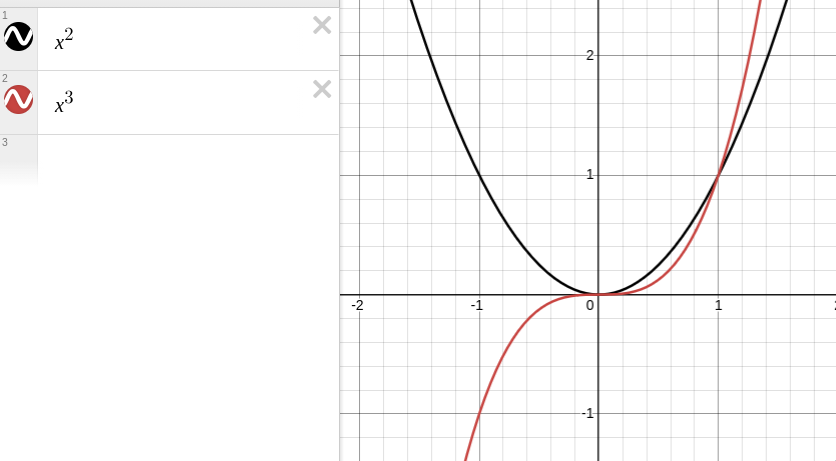
\includegraphics[width=0.6\textwidth]{pictures/mocnine_funkce.png} 
    \caption*{}
\end{figure}
\subsubsection*{Odmocninné funkce}
Tyto funkce mají předpis $y = x^\frac{1}{n}, n \in \mathbb{N}$ neboli $y = \sqrt[n]{x}, n \in
\mathbb{N}$. Tyto funkce jsou také velice rozdílné podle toho, zda je $n$ liché nebo sudé.

Pokud je $n$ sudé, definiční obor je $D(f) = \langle 0, \infty)$ a obor hodnot je $H(f) = \langle 0,
\infty)$. Funkce je rostoucí a konkávní. Tato funkce je inverzní s prvním kvadrantem mocninné funkce
se stejným $n$.

Pokud je $n$ liché definiční obor a obor hodnot jsou všechna reálná čísla. Tato funkce má inflexní
bod v $[0, 0]$. Funkce je lichá a inverzní k mocninné funkci se stejným exponentem a odmocnitelem.
\begin{figure}[H] 
    \centering    
    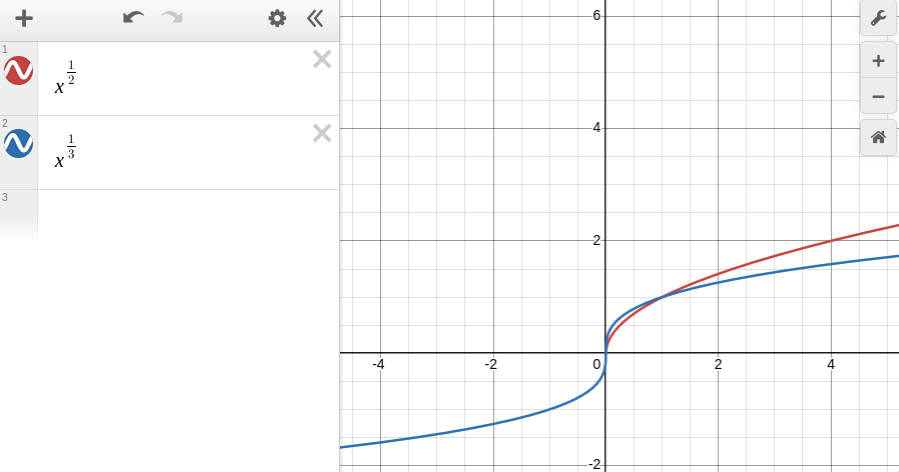
\includegraphics[width=0.6\textwidth]{pictures/odmocninne_funkce.png} 
    \caption*{}
\end{figure}
\subsubsection*{Mocniné funkce se záporným celým mocnitelem}
Tyto funkce mají předpis $y = x^{-n}, n \in \mathbb{N}$ neboli $y = \frac{1}{x^n}, n \in \mathbb{N}$.
Definiční obor těchto funkcí je $D(f) = \mathbb{R} \setminus \{0\}$. Tyto funkce se také chovají jinak
s ohledem na to jestli je $n$ sudé nebo liché číslo.

Pokud je $n$ sudé číslo, funkce je sudá a konvexní. Její obor hodnot je $H(f) = (0, \infty)$. Funkce
je rostoucí na intervalu $(-\infty, 0)$ a klesající na intervalu $(0, \infty)$.

Pokud je $n$ liché číslo, funkce je lichá a její graf se nazývá hyperbola. Obor hodnot je $H(f) =
\mathbb{R} \setminus \{0\}$. Funkce klesá na intervalu $(-\infty, 0)$ a $(0, \infty)$. Pozor, nedá
se říct, že funkce je klesající.
\begin{figure}[H] 
    \centering    
    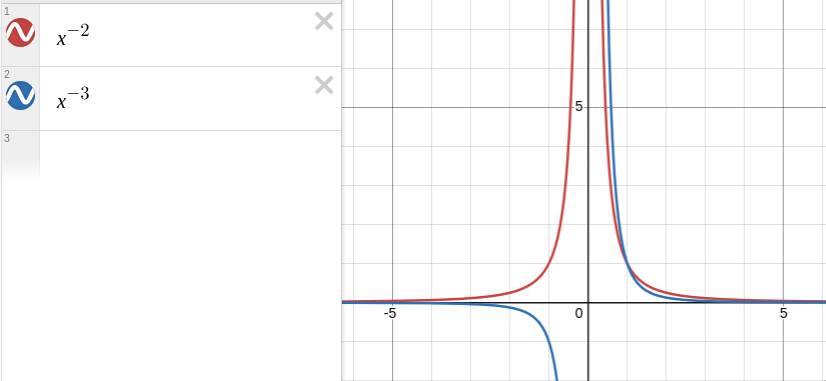
\includegraphics[width=0.6\textwidth]{pictures/mocnine_funkce_minus.png} 
    \caption*{}
\end{figure}
\subsubsection*{Lineární lomená funkce}
Tato funkce má předpis $y = \frac{ax + b}{cx + d}$. Pro lepší práci s ní se využije dělení
mnohočlenem aby vzniklo $y = \frac{k}{x-x_0} + y_0$. $D(f) = \mathbb{R} \setminus \{\frac{-d}{c}\},
H(f) = \mathbb{R} \setminus \{\frac{a}{c}\}$. Lineární lomená funkce je prostá. 
\begin{figure}[H] 
    \centering    
    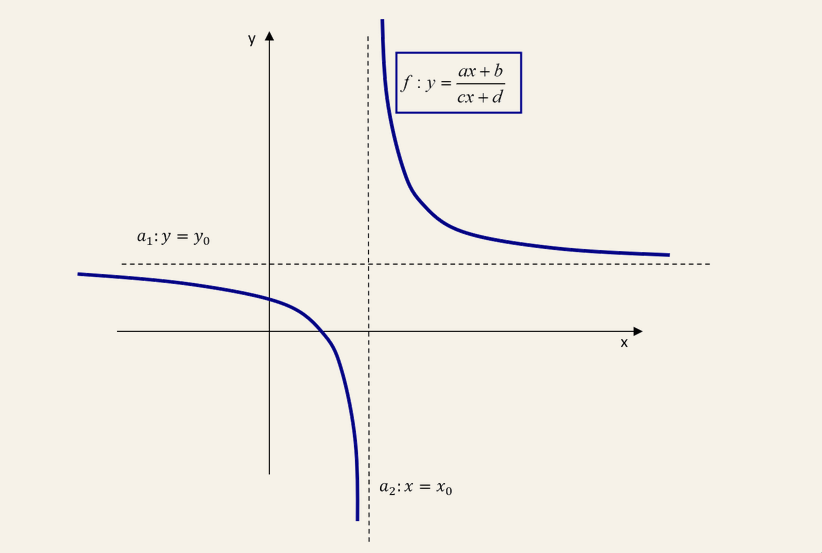
\includegraphics[width=0.6\textwidth]{pictures/linearni_lomena.png} 
    \caption*{}
\end{figure}
\end{document}
